\section{Network inference with GGM}

\begin{frame}
  \frametitle{Some families of methods for network reconstruction}

  \begin{block}{Test-based methods}
    \begin{itemize}
    \item Tests the nullity of each entries 
    \item Combinatorial problem when $p>30$ \dots
    \end{itemize}    
  \end{block}
  
  \vfill

  \begin{block}{\alert{Sparsity-inducing regularization methods}}
    \begin{itemize}
    \item induce sparsity with the $\ell_1$-norm penalization
    \item Use results from convex optimization
    \item Versatile and computationally efficient
    \end{itemize}
  \end{block}

  \vfill

  \begin{block}{Bayesian methods}
    \begin{itemize}
    \item Compute the posterior probability of each edge
    \item Usually more computationally demanding
    \item For special graphs, computation gets easier
    \end{itemize}
  \end{block}
  
\end{frame}

\pgfdeclareimage[height=0.8\textheight]{sparsity1}{figures/sparsity_1}
\pgfdeclareimage[height=0.8\textheight]{sparsity2}{figures/sparsity_2}
\pgfdeclareimage[height=0.375\textheight]{sparsity4}{figures/sparsity_4}

\begin{frame}
  \frametitle{Inference: maximum likelihood estimator}
  \framesubtitle{The natural approach for parametric statistics}
  
  Let   $X$  be  a   random  vector   with  distribution   defined  by
  $f_{X}(x;\boldsymbol\Theta)$,  where   $\boldsymbol\Theta$  are  the
  model parameters.

  \vfill

  \begin{block}{Maximum likelihood estimator}
    \begin{equation*}
      \hat{\boldsymbol\Theta}      =      \argmax_{\boldsymbol\Theta}
      \ell(\boldsymbol\Theta; \mathbf{X})
    \end{equation*} 
    where  $\ell$ is  the log  likelihood, a  function  of the
    parameters:
    \begin{equation*}
      \ell(\boldsymbol\Theta;      \mathbf{X})      =     \log
      \prod_{i=1}^n f_{X}(\mathbf{x}_i;\boldsymbol\Theta),
    \end{equation*}
    where $\mathbf{x}_i$ is the $i$th row of $\mathbf{X}$.
  \end{block}
  
  \vfill
  
  \begin{block}{Remarks}
    \begin{itemize}
    \item This a convex optimization problem,
    \item We just need to detect non zero coefficients in $\boldsymbol\Theta$
    \end{itemize}
  \end{block}
  
\end{frame}

\begin{frame}
  \frametitle{The multivariate Gaussian log-likelihood }
  
  Let  $\mathbf{S}  =  n^{-1}\mathbf{X}^\intercal \mathbf{X}$  be  the
  empirical variance-covariance  matrix: $\mathbf{S}$ is  a sufficient
  statistic of $ \boldsymbol\Theta$.

  \vfill

  \begin{block}{The log-likelihood}
    \begin{equation*}
      \ell(\boldsymbol\Theta; \mathbf{S}) =
      \frac{n}{2}     \log    \det     (\boldsymbol\Theta)  - \frac{n}{2}
      \mathrm{Trace}(\mathbf{S} \boldsymbol\Theta) + \frac{n}{2}\log(2\pi).
    \end{equation*}
  \end{block}
  
  \vfill
  
  \begin{itemize}
  \item[$\rightsquigarrow$]    The     MLE    $=\mathbf{S}^{-1}$    of
    $\boldsymbol\Theta$ is not defined for $n< p$ and never sparse.
  \item[$\rightsquigarrow$] The need for regularization is huge.
  \end{itemize}
\end{frame}

\begin{frame}
  \frametitle{A Geometric View of Shrinkage}
  \framesubtitle{Constrained Optimization}

  \begin{overlayarea}{\textwidth}{\textheight}
    \begin{columns}
      \begin{column}{0.475\textwidth}
        \begin{tikzpicture}
          \only<1>{%
            \node (Surf) at (0,0) {\pgfuseimage{sparsity1}}
            node     at    (Surf.west)    [rotate=90,yshift=5mm]
            {$L(\theta_1,\theta_2;\mathbf{X})$}
            node at (Surf.south west) [xshift=5mm,yshift=5mm]{$\theta_2$}
            node at (Surf.south east) [xshift=-7.5mm,yshift=2.5mm]{$\theta_1$};
          }
          \only<2>{%
            \node (Surf2) at (0,0) {\pgfuseimage{sparsity2}}
            node    at    (Surf2.west)    [rotate=90,yshift=5mm]
            {$L(\theta_1,\theta_2;\mathbf{X})$}
            node at (Surf2.south west) [xshift=5mm,yshift=5mm]{$\theta_2$}
            node at (Surf2.south east) [xshift=-7.5mm,yshift=2.5mm]{$\theta_1$};
          }
          \only<3->{%
            \node (titi) at (0,0) {\phantom{titi}};
            \node (Surf3) at (0,-4.5) {\pgfuseimage{sparsity4}}
            node at (Surf3.west) [rotate=90,yshift=2.5mm] {$\theta_2$}
            node at (Surf3.south) [yshift=-2.5mm] {$\theta_1$};
          }
        \end{tikzpicture}
      \end{column}
      \begin{column}{0.55\textwidth}
        \only<1>{%
          We basically want to solve a problem of the form
          \begin{equation*}
            \maximize_{\theta_1,\theta_2} \ell(\theta_1,\theta_2;\mathbf{X})
          \end{equation*}
          where $\ell$ is typically a concave likelihood function.
        }
        \only<2->{%
          \begin{equation*}
            \left\{\begin{array}{ll}
                \displaystyle    \maximize_{\theta_1,\theta_2}   &
                \ell(\theta_1,\theta_2;\mathbf{X})\\
                \mathrm{s.t.} & \Omega(\theta_1,\theta_2) \leq c
              \end{array}\right.,
          \end{equation*}
          where  $\Omega$  defines  a  domain  that  \textit{constrains}
          $\boldsymbol\beta$.

          \begin{center}
            How shall we define $\Omega$ ?
          \end{center}
        }
      \end{column}
    \end{columns}
  \end{overlayarea}
\end{frame}

\begin{frame}
  \frametitle{The Lasso}
  \framesubtitle{Least Absolute Shrinkage and Selection Operator}

  \begin{block}{Idea}
    Suggest  an admissible  set that  induces  \alert{sparsity} (force
    several entries to exactly zero in $\hat{\bbeta}$).
  \end{block}

  \vfill

  \begin{overlayarea}{\textwidth}{.4\textheight}
    \begin{columns}
      \begin{column}[c]{.6\textwidth}
        \begin{block}{Lasso as a regularization problem}
          The Lasso estimate of $\bbeta$ is the solution to
          \begin{equation*}
            \hat{\btheta}^{\text{lasso}}     =    \argmin_{\btheta}
            -\ell(\btheta),  \quad   \text{s.t.  }  \sum_{j=1}^p
            \left|\theta_j\right|
            \leq s,
          \end{equation*}
          where $s$ is a shrinkage factor.
        \end{block}
      \end{column}
      \begin{column}{.3\textwidth}
        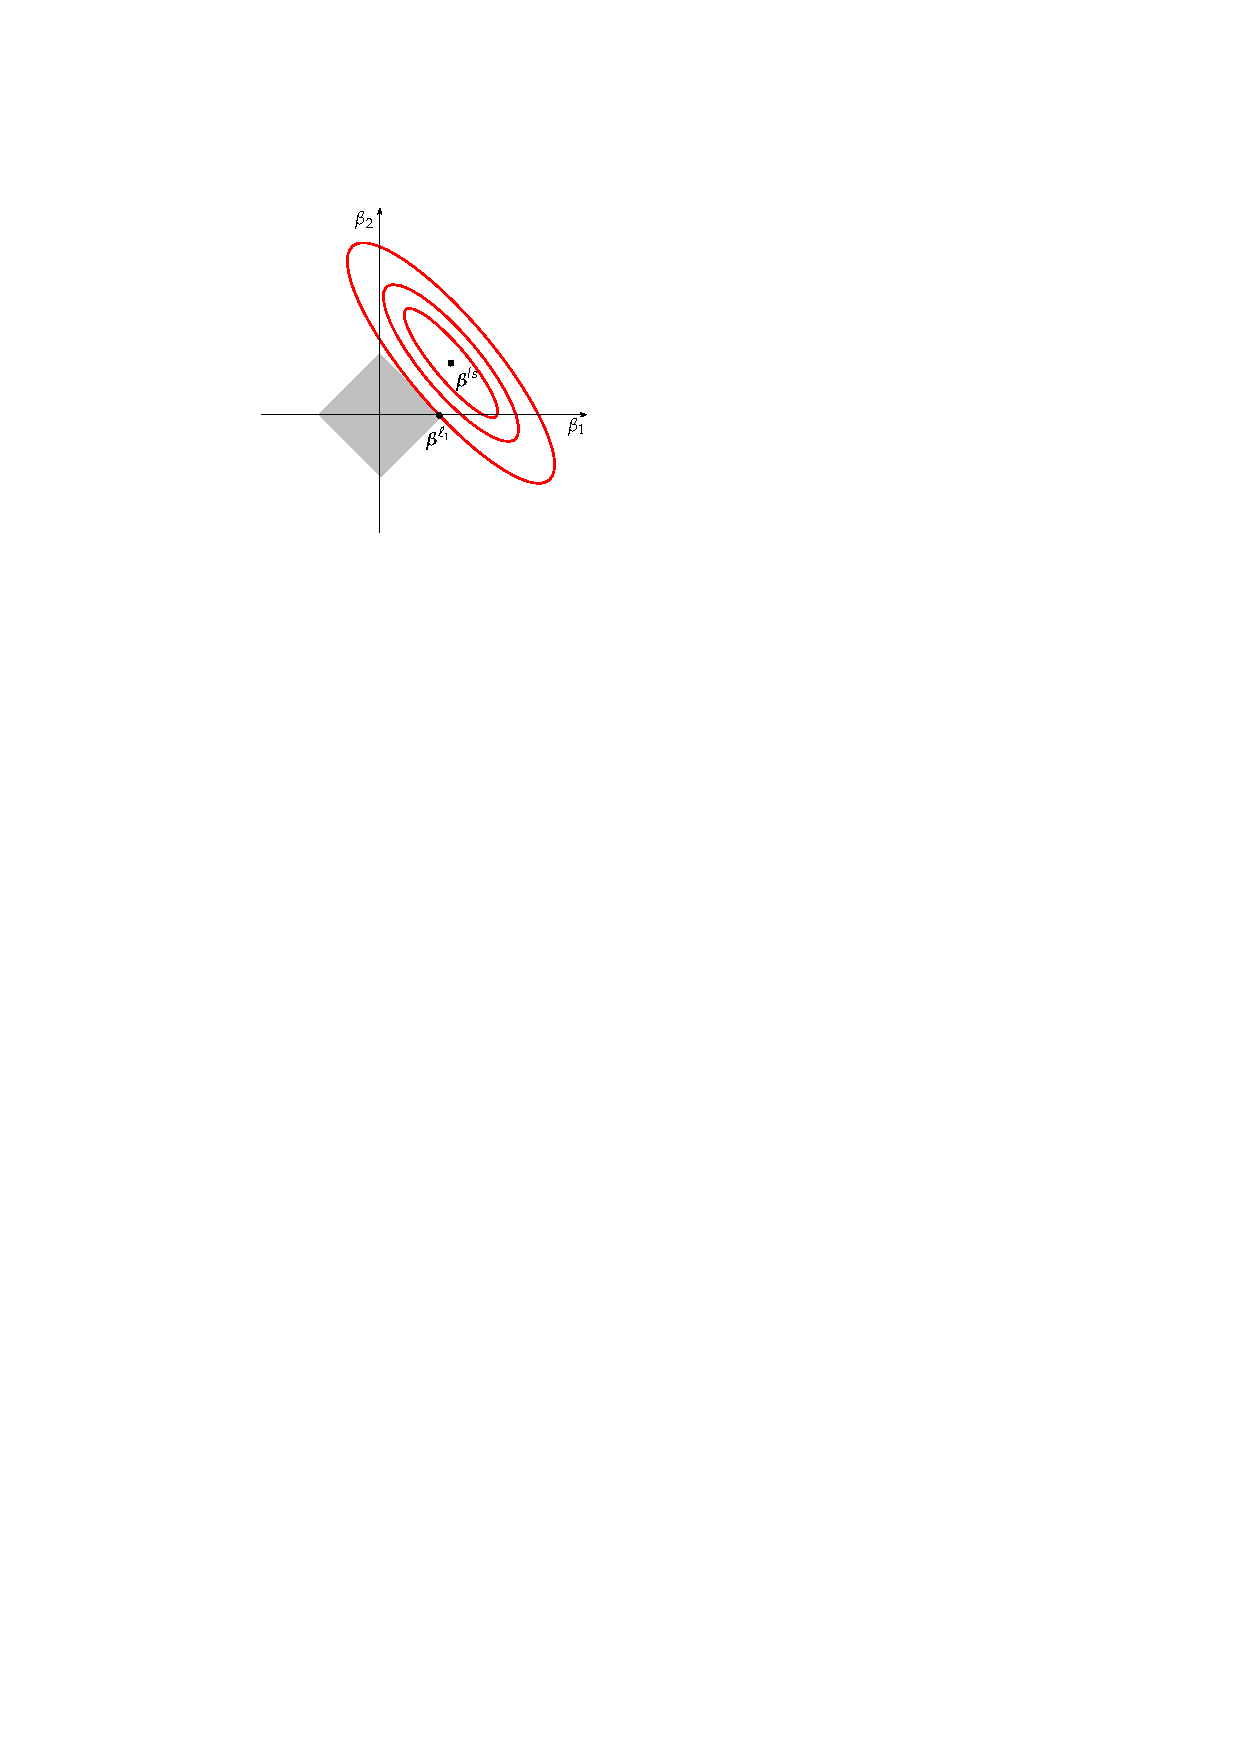
\includegraphics[width=\textwidth]{figures/lasso_set}
      \end{column}
    \end{columns}
  \end{overlayarea}

\end{frame}

\begin{frame}
  \frametitle{Insights: 2-dimensional example with the square loss}

  \begin{overlayarea}{\textwidth}{\textheight}

    \begin{equation*}
      \sum_{i=1}^n (y_i-x_i^1\theta_1 - x_i^2\theta_2)^2, \qquad
      \only<1>{\text{no constraints}}
      \only<2>{\text{s.t. } |\theta_1| + |\theta_2| < 0.75}
      \only<3>{\text{s.t. } |\theta_1| + |\theta_2| < 0.66}
      \only<4>{\text{s.t. } |\theta_1| + |\theta_2| < 0.4}
      \only<5>{\text{s.t. } |\theta_1| + |\theta_2| < 0.2}
      \only<6>{\text{s.t. } |\theta_1| + |\theta_2| < 0.0743}
    \end{equation*}

  \vspace{-.75cm}

    \includegraphics<1>[width=.9\textwidth]{dess11}
    \includegraphics<2>[width=.9\textwidth]{dess12}
    \includegraphics<3>[width=.9\textwidth]{dess13}
    \includegraphics<4>[width=.9\textwidth]{dess14}
    \includegraphics<5>[width=.9\textwidth]{dess15}
    \includegraphics<6>[width=.9\textwidth]{dess16}

  \end{overlayarea}

\end{frame}

\begin{frame}
  \frametitle{Application to GGM: the "Graphical-Lasso"} 

  \begin{block}{A penalized likelihood approach}
    \vspace{-1em}
    \begin{equation*}
      \hat{\bTheta}_\lambda=\argmax_{\bTheta \in \mathbb{S}_+}
      \ell(\bTheta;\mathbf{X})-\lambda
      \|\bTheta\|_{\ell_1}
    \end{equation*}
  where
  \begin{itemize}
  \item $\mathcal{\ell}$ is the model log-likelihood,
  \item $\|\cdot\|_{\ell_1}$ is a \alert{penalty function} tuned by
    $\lambda>0$. 
    \vfill
      \begin{enumerate}
      \item \textit{regularization} (needed when $n \ll p$), 
      \item \textit{selection} (sparsity induced by the $\ell_1$-norm),
      \end{enumerate}
    \item     solved    in     \texttt{R}-packages    \textbf{glasso},
      \textbf{quic}, \textbf{huge} ($\mathcal{O}(p^3)$)
  \end{itemize}
\end{block}

\end{frame}

\begin{frame}
  \frametitle{Application to GGM: "Neighborhood selection"} 

  A close cousin, thank to the relationship between Gaussian vector and linear regression
  
  \textcolor{gray}{
  Remember that
  \begin{equation*}
    X_i | X_{ \setminus i} = \sum_{\alert{j \in \text{neighbors}(i)}} \beta_j X_j + \varepsilon_i
    \quad         \text{with         }         \beta_j         =
    -\frac{\Theta_{ij}}{\Theta_{ii}}.
  \end{equation*}
  }
  
  \begin{block}{A penalized least-square approach}
    Let $\bX_i$ be the $i$th column of the data matrix (i.e data associated to variable (gene) $i$), and $\bX_{\backslash i}$ deprived of colmun $i$. We select the neighbors of variable $i$ by solving
    \begin{equation*}
      \widehat{\boldsymbol\beta}^{(i)} = \argmin_{\boldsymbol\beta \in \mathbb{R}^{p-1} }
      \frac{1}{n} \left\| \mathbf{X}_i - \mathbf{X}_{\backslash i} \,
        {\boldsymbol\beta} \right\|_2^2 + \lambda \left\| {\boldsymbol\beta} \right\|_{1}
    \end{equation*}

    \begin{itemize}
    \item[\textcolor{red}{$-$}] not symmetric, not positive-definite
    \item[\textcolor{green}{$+$}] $p$
      Lasso solved with Lars-like algorithms ($\mathcal{O}(npd)$ for $d$ neighbors).
    \end{itemize}

\end{block}

\end{frame}


% \begin{frame}
%   \frametitle{Network inference for count data}
%   \framesubtitle{Data transformation}
% 
%   Consider $\bX = (X^1,\dots,X^n)$ some count data with size $n\times p$. 
% 
%   \begin{block}{Simple transformation}
%     Often surprisingly efficients
%     \begin{itemize}
%     \item log transformation $\log(1 + \bX)$
%     \item compute $\boldsymbol S_n$ by means of \alert{Spearman's correlation}
%     \end{itemize}
%   \end{block}
% 
%   \vfill
% 
%   \begin{block}{Non paranormal transformation (Liu et al 2009)}
%     The random vector $X$ has non-paranormal distribution if there exist \[f(X)=f(X_1,\dots, X_p)
%     \sim\mathcal{N}(\boldsymbol\mu,\boldsymbol\Theta^{-1}).\]
%     \begin{itemize}
%     \item Distribution of $X$  is a  \alert{Gaussian copula} if  $f$ is
%       monotone differentiable
%     \item    $X_i    \indep    X_j   |    X_{\backslash    i,j}$    iff
%       $\boldsymbol\Theta_{ij} = 0$.
%     \end{itemize}
%   \end{block}
% 
% \end{frame}

% \begin{frame}
%   \frametitle{Network inference for count data}
%   \framesubtitle{Poisson graphical models} 
%   
%   \begin{block}{Poisson graphical Lasso (Allen et al, 2012)}
%     Assuming  that   $X_j  |   X_k  \sim   \mathcal{P}(\exp(\beta_j  +
%     \sum_{j\neq k} \beta_k X_k ))$
%     \begin{equation*}
%       \hat{\bbeta}            \argmin_{\hat{\bbeta}\in\Rset^p}           
%       \left\{ -\sum_{i=1}^n\sum_{k\neq j} X_{ij} X_{ik}\beta_k -
%         \exp\{X_{ik}\beta_k \} \right\} + \lambda \|\bbeta \|_1.
%     \end{equation*}
%     \begin{itemize}
%     \item[$\rightsquigarrow$]    \alert{Log-linear    version}    of
%       neighborhood selection
%     \item[$\rightsquigarrow$]  Other extensions  in Yang  et al,  2014
%       (truncated Poisson).
%     \end{itemize}
%   \end{block}
% 
%   \vfill
%   
%   \begin{itemize}
%   \item[\textcolor{green}{$+$}] Better performance than GGM\dots
%   \item[\textcolor{red}{$-$}] \dots on simulated Poisson data
%   \item[\textcolor{red}{$-$}] Computationally less efficient
%   \end{itemize}
%   
% \end{frame}
% 
% \begin{frame}
%   \frametitle{Dealing with the growing number of feature}
%   
%   \begin{block}{Problem}
%     The number of OTU $p$ may be huge in metagenomics studies 
%     \begin{itemize}
%     \item Statistical limitation (depends on $d,n$)
%     \item Computational limitation (depends on your time but max. 1e6)
%     \end{itemize}
%   \end{block}
% 
%   \vfill
%   
%   \begin{block}{How should we limit the size of the problem?}
%     \begin{itemize}
%     \item Screening (discarding of irrelevant variables)
%     \item Clustering (aggregation of similar actors)
%     \end{itemize}
%     $\rightsquigarrow$ How does this affect the inferred networks?
%   \end{block}
%     
% \end{frame}
